\documentclass[alsotrans]{beamerswitch}
\usepackage{sdp}

\begin{filecontents*}{datastruct.bib}
@book{wirth1984data,
  title={Algorithms + data structures = programs},
  author={Niklaus Wirth},
  year={1976},
  publisher={Englewood Cliffs, N.J. : Prentice-Hall}
}
\end{filecontents*}

\title[СД+А=П]{Структури от данни\\+\\алгоритми\\=\\програми}

\date{7 октомври 2019 г.}

\begin{document}

\begin{frame}
  \titlepage
\end{frame}

\begin{frame}
  \nocite{*}
  \bibliographystyle{plain}
  \bibliography{datastruct}
\end{frame}

\section{Типове и структури}

\begin{frame}
  \frametitle{Типове данни (ТД)}

  Инструмент за класификация на данните, характеризиращ се с:
  \begin{itemize}
  \item множество от стойности
  \item операции над стойностите
  \end{itemize}
  \vspace{2ex}
  \pause
  \alert{За какво служат типовете?}
\end{frame}

\begin{frame}
  \frametitle{Типове данни в C++}

  \textbf{Примитивни:}
  \begin{itemize}
  \item булев (\lst{bool})
  \item целочислен (\lst{short}, \lst{int}, \lst{long}, \lst{unsigned})
  \item числа с плаваща запетая (\lst{float}, \lst{double})
  \item символен (\lst{char})
  \item указател (\tt*)
  \item псевдоним (\tt\&)
  \end{itemize}

  \textbf{Съставни:}
  \begin{itemize}
  \item масив (\lst{[]})
  \item структура / запис (\lst{struct})
  \item клас (\lst{class})
  \end{itemize}
\end{frame}

\begin{frame}
  \frametitle{Структури от данни (СД)}

  \begin{itemize}[<+->]
  \item СД са схеми за организация на даден вид данни в паметта на компютъра
    \begin{itemize}
    \item обикновено с цел ефективност
    \end{itemize}
  \item Всеки съставен ТД в частност може да се разглежда като СД
    \begin{itemize}
    \item \textbf{Пример:} \lst{int[]} е ТД масив от елементи от тип \lst{int} и може да се разглежда като СД, която представя редица от цели числа последователно в паметта
    \end{itemize}
  \item СД често се реализират чрез потребителски дефинирани ТД
    \begin{itemize}
    \item \textbf{Пример:} СД ``разширяващ се стек'' може да се реализира с ТД \lst{class ResizingStack}
    \end{itemize}
  \end{itemize}
\end{frame}

\begin{frame}
  \frametitle{Абстрактен тип данни (АТД)}

  \begin{itemize}[<+->]
  \item Формален модел на ТД или СД
    \begin{itemize}[<.->]
    \item Множество от стойности
    \item Описание на имената и вида на операциите
    \item Описание на поведението и свойствата на операциите
    \end{itemize}
  \item Не налага конкретна организация на паметта
    \begin{itemize}[<.->]
    \item (за разлика от СД)
    \end{itemize}
  \item Не налага конкретно представяне със средствата на някакъв език
    \begin{itemize}[<.->]
    \item (за разлика от ТД)
    \end{itemize}
  \item Допуска една или повече реализации
  \item \alert{Какви са предимствата на АТД?}
  \end{itemize}
\end{frame}

\begin{frame}
  \frametitle{Видове описания на СД}

  \textbf{Логическо описание (АТД)}
  \begin{itemize}
  \item същност и предназначение
  \item компоненти
  \item операции
  \item свойства на операциите
  \end{itemize}
  \vspace{1em}
  \pause
  \textbf{Физическо описание}
  \begin{itemize}
  \item организация на паметта
  \item представяне с един или повече ТД
  \item реализация на операциите
  \end{itemize}
\end{frame}

\begin{frame}
  \frametitle{Видове СД}

  \begin{itemize}[<+->]
  \item Според вида на комопонентите си
    \begin{itemize}[<.->]
    \item хомогенни (масив)
    \item хетерогенни (структура)
    \end{itemize}
  \item Според способността за промяна на размера
    \begin{itemize}[<.->]
    \item статични (статичен масив)
    \item динамични (разширяващ се масив)
    \end{itemize}
  \item Според връзките между данните
    \begin{itemize}[<.->]
    \item линейни (свързан списък)
    \item разклонени (дърво)
    \item мрежови (граф)
    \end{itemize}
  \end{itemize}
\end{frame}

\section{Алгоритми}

\begin{frame}
  \frametitle{Какво е алгоритъм?}

  \pause
  \textbf{Неформално:}\\
  Добре дефиниран набор от инструкции за извършване на дадено пресмятане.\\[2em]
  \pause
  \textbf{Формално:}\\
  Машина на Тюринг (например)
\end{frame}

\begin{frame}
  \frametitle{Масови задачи}

  \begin{itemize}[<+->]
  \item \textbf{Масова задача:} общ изчислителен проблем, който може да бъде формулиран за входни данни с произволен размер
    \begin{itemize}
    \item \textbf{Пример:} подреждане на елементи на масив във възходящ ред (сортиране)
    \end{itemize}
  \item Алгоритъмът като решение на масова задача
  \item Една масова задача може да има много възможни решения
  \item \alert{Как да сравняваме алгоритмите?}
  \item Добре е да имаме мярка за ефективността на алгоритъма
  \item Такава мярка обикновено се нарича \textbf{сложност на алгоритъма}
  \end{itemize}
\end{frame}

\begin{frame}
  \frametitle{Сложност на алгоритъм}

  Алгоритъм е по-ефективен, ако има нужда от по-малко ресурс.\\
  \pause
  Видове сложност:
  \begin{itemize}[<+->]
  \item \textbf{времева} --- оценка на времето за изпълнение на алгоритъма
  \item \textbf{пространствена} --- оценка на паметта използвана от алгоритъма
  \end{itemize}
  \onslide<+->
  \vspace{1em}
  Как да оценим колко ресурс използва даден алгоритъм?\\[1em]
  \begin{itemize}[<+->]
  \item брой процесорни инструкции и брой байтове?
    \begin{itemize}
    \item не знаем на какъв процесор ще се изпълнява програмата!
    \end{itemize}
  \item брой ``атомарни операции'' и брой ``единици памет''?
    \begin{itemize}
    \item зависи колко големи данни подадем на алгоритъма
    \end{itemize}
  \item функция на броя операции или променливи в зависимост от големината на входа?
    \begin{itemize}
    \item точният брой може да варира в зависимост от конкретната реализация или език за програмиране
    \item но варирането \textbf{не трябва да зависи от големината на входа}
    \end{itemize}
  \end{itemize}
\end{frame}

\begin{frame}
  \frametitle{Асимптотична сложност}

  Оценка на нарастването на функцията на сложност при \alert<8>{нарастването} на големината на данните за обработка.\\
  \pause
  \textbf{Пример 1:}
  \begin{itemize}[<+->]
  \item Нека имаме два алгоритъма $A$ и $B$.
  \item При вход с големина $n$ двата алгоритъма изпълняват съответно $f_A(n) = n^2 + 3n$ операции и
    $f_B(n) = 100n + 5$ операции.
  \item<+-|alert@+-> Кой от двата алгоритъма е по-бърз
  \item $f_A(10) = 130,\quad f_B(10) = 1005$
  \item $f_A(100) = 10300,\quad f_B(1000) = 10005$
  \item $f_A(1000) = 1003000,\quad f_B(1000) = 100005$
  \item Но нас ни интересува какво се случва при \alert{големи данни ($n \to \infty$)}!
  \item За големи данни $B$ е все по-бърз в сравнение с $A$
  \item За големи данни $f_A(n) \approx n^2$, $f_B(n) \approx 100n$
  \end{itemize}
\end{frame}

\begin{frame}
  \frametitle{Асимптотична сложност}

  Оценка на \alert<6>{нарастването} на функцията на сложност при нарастването на големината на данните за обработка.\\
  \textbf{Пример 2:}
  \begin{itemize}[<+->]
  \item Нека $C$ и $D$ имат сложности $f_C(n) = 2n^2 + 10n$, $f_D(n) = 3n^2$.
  \item $f_C(5) = 100,\quad f_D(5)= 75$
  \item $f_C(10) = f_D(10) = 300$
  \item $f_C(20) = 1000,\quad f_D(20) = 1200$
  \item Изобщо, за $n \geq 10$ имаме $f_C(n) \leq f_D(n)$
  \item Но нас ни интересува \alert{нарастването} на функцията!
  \item $f_A(2n) = 4n^2 + 6n \approx \alert4f_A(n), \quad f_B(2n) = 200n + 5 \approx \alert2f_B(n)$
  \item $f_C(2n) \approx \alert4f_C(n),\quad f_D(2n) \approx \alert4f_D(n)$
  \item $A, C, D$ се усложняват с еднаква скорост с увеличаване на $n$, а $B$ се усложнява по-бавно от тях.
  \item Искаме класификация, която нарежда $f_A, f_C$ и $f_D$ на едно и също ниво, а $f_B$ по-ниско.
  \end{itemize}
\end{frame}

\begin{frame}
  \frametitle{$O$-нотация}

  \textbf{Проблем:} искаме да категоризираме функциите относно поведението им при големи стойности, т.е. техния ``порядък''\\
  \textbf{Решение:} дефинираме класове от функции.
  \pause
  Нека $f, g : \mathbb N \to \mathbb N$.
  \begin{eqnarray*}
    f \in O(g) &\Longleftrightarrow& \exists C \exists k \forall n \geq k\;(0 \leq f(n) \leq C\cdot g(n))\\
    && (\text{\small $f$ расте \textbf{по-бавно} от $g$})\\
    \pause
    f \in \Omega(g) &\Longleftrightarrow & \exists C \exists k \forall n \geq k\;(0 \leq C\cdot g(n) \leq f(n))\\
    && (\text{\small $f$ расте \textbf{по-бързо} от $g$})
  \end{eqnarray*}
  \pause
  Лесно се вижда, че $f\in O(g) \Leftrightarrow g\in \Omega(f)$.
  \pause
  \begin{equation*}
    f\in \theta(g) \Longleftrightarrow \exists C_1 \exists C_2 \exists k \forall n \geq k\;(0 \leq C_1\cdot g(n) \leq f(n) \leq C_2\cdot g(n))
  \end{equation*}
  \pause
  Лесно се вижда, че $\Theta(g) = O(g) \cap \Omega(g)$.
\end{frame}

\begin{frame}
  \frametitle{$O$-нотация: примери}

  \begin{itemize}[<+->]
  \item $f \in \Theta(f) = O(f) \cap \Omega(f)$
  \item $1000n^2 \in O(n^3)$ \onslide<+-> (при $C = 1000$ е вярно, че $1000n^2 \leq 1000n^3$)
  \item $3n^2 + 100 \in \Theta(n^2)$ \onslide<+->, защото при $C_1 = 1, C_2 = 4, k = 10$ е вярно, че
    \begin{equation*}
      \forall n \geq 10\;(0 \leq n^2 \leq 3n^2 + 100 \leq 4n^2)
    \end{equation*}
  \item $2^n \in O(3^n)$, $\log_2 (n) \in \Theta(log_{10}(n))$
    \begin{itemize}
    \item обикновено бележим просто $\log n$, понеже основата няма значение
    \end{itemize}
  \item $\log n \in O(n^{0.001})$, $n^{1000}\in O(1.001^n)$
  \item $\forall C (C \in \Theta(1))$, $O(1) = \Theta(1)$, $\Omega(1) = \mathbb N^{\mathbb N}$
  \end{itemize}
\end{frame}

\begin{frame}
  \frametitle{$O$-нотация: често използвани сложности}
  \begin{center}
    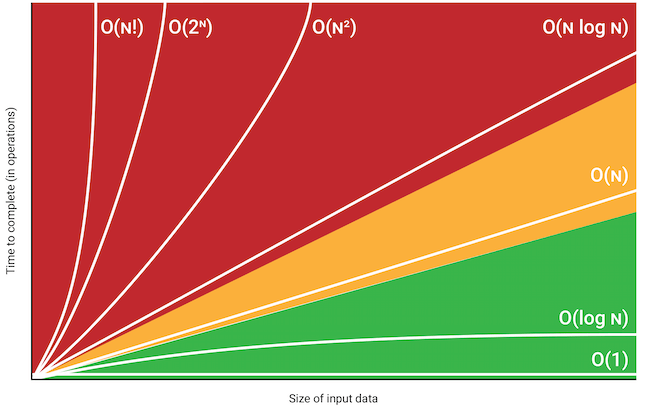
\includegraphics[height=0.7\textheight]{images/big-o.png}\\
    \imageUntitledAttr{Daniel Miessler}{https://danielmiessler.com/study/big-o-notation/}{CC BY-SA 2.0}
  \end{center}
\end{frame}

\begin{frame}
  \frametitle{Видове сложност}

  \begin{itemize}[<+->]
  \item В най-лошия случай (песимистична)
    \begin{itemize}
    \item Какъв е максималният възможен брой операции (единици памет), които могат да са нужни на алгоритъма, за да реши задачата?
    \end{itemize}

  \item В най-добрия случай (оптимистична)
    \begin{itemize}
    \item Какъв е минималният възможен брой операции (единици памет), които може да извърши (използва) алгоритъмът, за да реши задачата?
    \end{itemize}

  \item В средния случай (средна)
    \begin{itemize}
    \item Ако считаме, че всеки възможен вход е равновероятен, какво е ``средното аритметично'' на броя операции (единици памет), които трябват при всички възможни входове?
    \end{itemize}

  \item При многократно изпълнение (амортизирана)
    \begin{itemize}
    \item Ако алгоритъмът ще се извиква няколко пъти в рамките на дадена програма, колко операции (единици памет) средно ще са му необходими за едно извикване?
    \end{itemize}
  \end{itemize}

\end{frame}

\begin{frame}[fragile]
  \frametitle{Пресмятане на сложност: пример}

  % TODO: разписване на пресмятането на сложност
\begin{lstlisting}
for(int i = 0; i < n-1; i++)
  for(int j = n-2; j >= i; j--)
    if (a[j] > a[j+1]) {
      double x = a[j];
      a[j] = a[j+1];
      a[j+1]= x;
    }
\end{lstlisting}

Да се оценят песимистична, оптимистична и средна времева сложност.
\end{frame}

\section{STL}

\begin{frame}
  \frametitle{Standard Template Library (STL)}

  Библиотека от шаблони, реализираща стандартни структури от данни и алгоритми.

  \begin{itemize}
  \item част от C++ Standard Library
  \item основни компоненти
    \begin{itemize}
    \item алгоритми (\lst{<algorithm>})
    \item контейнери (\lst{<queue>}, \lst{<stack>}, \lst{<vector>}, \lst{<list>}, \lst{<map>}, \ldots)
    \item функционални обекти (\lst{<functional>})
    \end{itemize}
  \item базирана на идеята за генерично програмиране
  \item ефективност: дава гаранции за сложност на алгоритми и операции над СД
  \end{itemize}
\end{frame}

\end{document}
